\section{Theorie}

\subsection{Zielsetzung}

\noindent 
Das Ziel dieses Versuches ist die Untersuchung der effektiven Masse $m^*$ von Leitungselektronen in $\ce{GaAs}$ und $\ce{InGaAs}$. 
Dies geschieht über die Bestimmung der Faraday-Rotation einzelner Wellenlängen $\lambda$ in den Materialien.

\subsection{Bandstruktur und effektive Masse}
       

\noindent
Im Allgemeinen lassen sich die möglichen Energieniveaus von Elektronen in kristallinen Festkörpern über die Bandstruktur beschreiben. 
Dabei werden die über das Pauli-Prinzip möglichen Energieniveaus gegen den Wellenvektor $\vec{k}$ aufgetragen. 
Für eine sehr große Anzahl der Niveaus gehen die einzelnen Niveaus in kontinuierliche Bänder über.
Für eine nicht betrachtete Änderung der Wellenzahl $k$ sind die Bandkanten linear. 
Dies ist schematisch für verschiedene Materialien in Abbildung \ref{img:Band} dargestellt.\\\\

%\begin{figure}[H]
%    \centering
%    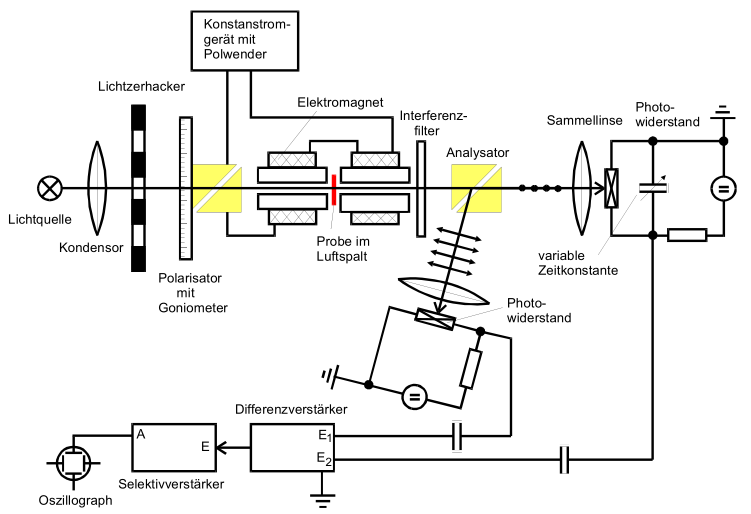
\includegraphics[width=0.7\textwidth]{latex/images/Aufbau.PNG}
%    \caption{Der schematische  \protect \cite{V46}.}
%    \label{img:Band}
%\end{figure}

\noindent
Für Metalle ist das Valenzband voll besetzt, im Leitungsband sind aber auch Niveaus gefüllt. 
Diese führen dazu, dass Metalle bei niedrigen Temperaturen leitfähig sind, da Elektronen höher energetische Niveaus annehmen können und damit beschleunigt werden können.
Für Halbleiter und Isolatoren ist das Valenzband voll besetzt, dass Leitungsband aber leer. Die Materialien können also nicht leiten, da die Elektronen ihre Niveaus nicht ändern können.
Bei Halbleitern ist die Bandlücke allerdings so klein, dass für große Temperaturen Elektronen in das Leitungsband wechseln können, wodurch das Material leitfähig wird.\\
Bei Raumtemperatur ist dieser Effektrelativ klein, lässt sich aber durch Dotierung des Materials erhöhen. Dabei ist zwischen $n$- und $p$-Dotierung zu unterscheiden.
Bei $n$-Dotierung werden Fremdatome die ein zusätzliches Valenzelektron besitzen, eingebracht. Diese sind die sogenannten Donatoren. 
Die Energieniveaus der zusätzlichen Elektronen sind dabei kurz unter der Bandkante angesiedelt, sodass weniger thermische Energie für Elektronen benötigt wird, 
um ins Leitungsband zu wechseln.
Dadurch wird bei Raumtemperatur schon eine signifikante Leitfähigkeit erreicht.\\
Für $p$-Dotierung wird ein Atom mit einer zusätzlichen Leerstelle, den sogenannten Akzeptoren eingebracht.
Deren Niveau ist knapp über der Valenzbandkante angesiedelt. 
Der Übergang in dieses Niveau benötigt weniger Energie, wodurch eine Leerstelle im Valenzband frei wird, die zu Lochleitfähigkeit führt.
Diese Niveaus sind in Abbildung \ref{img:dot} dargestellt. \\\\

%\begin{figure}[H]
%    \centering
%    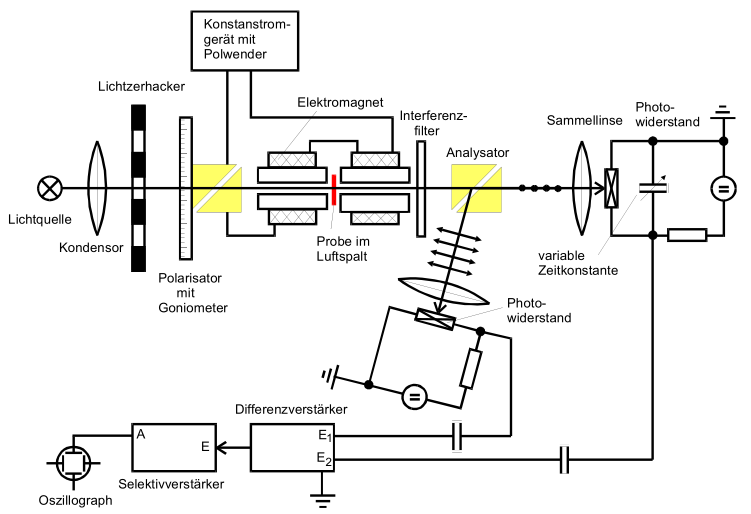
\includegraphics[width=0.7\textwidth]{latex/images/Aufbau.PNG}
%    \caption{Der schematische  \protect \cite{V46}.}
%    \label{img:dot}
%\end{figure}


\noindent
Um die Bewegung der Elektronen zu beschreiben wird das Konzept der effektiven Masse $m^*$ eingeführt. 
Dabei wird berücksichtigt, dass sich die Elektronen nicht in einem freien Gas bewegt, sondern in einem periodischen Potential. 
Dafür lässt sich für die Näherung in einem lokalen Minimum des Potentials, für die Beschleunigung der Elektronen nach Newton, die Gleichung
\begin{equation*}
    a = \frac{1}{\hslash^2}\frac{\symup{d}^2\epsilon}{\symup{d}k^2} \cdot qE 
\end{equation*} 
aufstellen. Dabei ist $a$ die Beschleunigung, $q$ die Ladung des Elektrons und $E$ das externe elektrische Feld.
Der Vergleich mit dem zweiten Newtonschen Gesetz ergibt dann
\begin{equation*}
    m^* =  \hbar^2 \frac{\symup{d}k^2}{\symup{d}^2\epsilon}\quad.
\end{equation*} 
Dabei ist $m^*$ in der Regel ein Tensor, da die effektive Masse richtungsabhängig sein kann.
Bei hinreichend hoher Symmetrie des Kristalls wird $m^*$ ein skalar. 



\subsection{Zirkulare Doppelbrechung}

\noindent Wenn ein linear polarisierter Lichtstrahl auf ein optisch aktives Medium fällt, dreht sich die Polarisationsebene beim Durchlaufen des Materials um den Winkel $\theta$.
Dies wird als zirkulare Doppelbrechung bezeichnet. Dies ist schematisch in Abbildung \ref{img:zirk} dargestellt.

\begin{figure}[H]
    \centering
    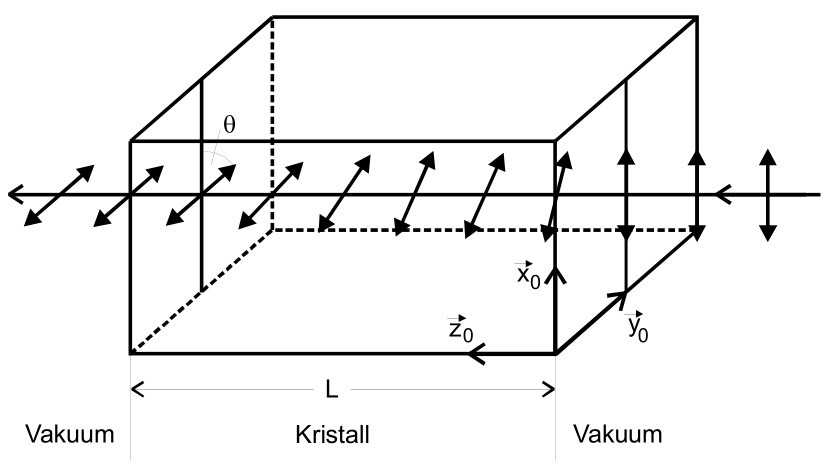
\includegraphics[width=0.7\textwidth]{latex/images/zirk.PNG}
    \caption{Eine schematische Darstellung der Drehung der Polarisationsebene in optisch aktiven Materialien  \protect \cite{anhang}.}
    \label{img:zirk}
\end{figure}

\noindent
Dieser Effekt kann damit erklärt werden, dass links- und rechts-polarisiertes Licht in Materialien unterschiedliche Phasengeschwindigkeiten besitzen können.
Und da eine linear polarisierte Welle als Superposition einer links- und rechts-polarisiertes Welle beschrieben werden kann, 
führen die unterschiedlichen Phasengeschwindigkeiten bis zum Austritt aus dem Material zu 
einer Drehung der Polarisationsebene.\\
Mathematisch lässt sich die Superposition der elektrischen Felder über 
\begin{equation*}
    E\left(z\right) = \frac{1}{2}\left(E_\text{L}+E_\text{R}\right)
\end{equation*}
beschreiben. 
Die Rotation berechnet sich dann über
\begin{equation}
    \theta = \frac{d}{2}\left(k_\text{R}-k_\text{L}\right) = \frac{d\omega}{2}\left(\frac{1}{v_\text{ph,R}}-\frac{1}{v_\text{ph, L}}\right) = \frac{d\omega}{2c}\left(n_\text{R}-n_\text{L}\right)
    \label{eqn:theta}
\end{equation} 
wobei für die Wellenzahlen $k_\t{L} \neq k_\t{R}$ gilt. 
Dabei ist $d$ die Dicke des Materials, $v_\t{ph} = \frac{\omega}{k}$ die Phasengeschwindigkeit und $n$ der Brechungsindex.\\
In Kristallen lässt sich die zirkulare Doppelbrechung darauf zurückführen, dass der Lichtstrahl Dipolmomente induzieren kann.
Diese entstehen durch Leitungselektronen die mit Atomrümpfen wechselwirken oder durch die Kerne selber.
Durch die einzelnen Dipole wird eine Gesamtpolarisation des Materials $\vec{P}$ hervorgerufen.
Für diese gilt
\begin{equation*}
    \vec{P} = \epsilon_0 \chi \vec{E} \quad,
\end{equation*}
mit $\epsilon_0$ als dielektrische Konstante und $\chi$ als elektrische Suszeptibilität. 
Im Allgemeinen, für anisotrope Kristalle, ist $\chi$ ein Tensor, der nur für Isotrope Kristalle zu einem Skalar wird.
Für doppelbrechende Materialien lässt er sich über
\begin{equation}
    \chi = \left( \begin{array}{rrr}\chi_\text{xx} & i\chi_\text{xy} & 0 \\-i\chi_\text{yx} & \chi_\text{yy} & 0\\0 & 0 & \chi_\text{zz}\\\end{array}\right)
    \label{eqn:chi}
\end{equation}
beschreiben. Mit Hilfe davon, der Wellengleichung einer ebenen Welle 
\begin{equation*}
    \vec{E}(\vec{r},t) = \vec{E}_0 \t{exp}\left(\vec k \vec r - \omega t\right)
\end{equation*}
und der dielektrischen Verschiebung
\begin{equation*}
    \vec D = \epsilon_0 \vec E + \vec P 
\end{equation*}
lässt sich der Ausdruck 
\begin{equation}
    k_\pm = \frac{\omega}{\t{c}} \sqrt{ \left(1 + \chi_{x,x}\right) \pm \chi_{x,y}}
    \label{eqn:k}
\end{equation}
für die Wellenzahlen der unterschiedlichen Polarisationsrichtungen herleiten.
Für die Phasengeschwindigkeiten bedeutet dies 
\begin{align*}
    v_\t{Ph,R} &= \frac{\t{c}}{\sqrt{ \left(1 + \chi_{x,x}\right) + \chi_{x,y}}}\\
    \intertext{und}
    v_\t{Ph,R} &= \frac{\t{c}}{\sqrt{ \left(1 + \chi_{x,x}\right) - \chi_{x,y}}} \quad .
\end{align*}
Über \autoref{eqn:k} und \autoref{eqn:theta} ergibt sich dann
\begin{equation*}
    \theta = \frac{d \omega}{\t{c}} \left(\left(1 + \chi_{x,x}\right) + \chi_{x,y} - \left(1 + \chi_{x,x}\right) - \chi_{x,y} \right)
\end{equation*}
was sich für kleine $\chi_{x,y}$ zu
\begin{equation*}
    \theta \approx \frac{d\omega}{2cn}\chi_\text{x,y}
\end{equation*}
nähern lässt.


\subsection{Der Faraday-Effekt}
  

\noindent
Für optisch inaktive Materialien gilt für die Nebendiagonalelemente $\chi_{i,j} = 0$, wodurch sie nicht zirkular doppelbrechend sind.
Allerdings lässt sich dies durch Anlegen eines externen Magnetfeldes parallel zur Ausbreitungsrichtung des Lichts ändern. 
Dort führt das elektromagnetische Feld des Lichts zu einer kreisförmigen Bewegung von Ladung im Material. Diese wiederum erzeugt selbst ein Magnefeld,
welches für eine Polarisationsrichtungen parallel zum externen Magnetfeld ist und für die andere entgegengesetzt. Dies führt zu einer Änderung der Phasengeschwindigkeiten der 
verschiedenen Polarisationen.\\
Für ein gebundenes Elektron lässt sich die Rotation über die Bewegungsgleichung
\begin{equation*}
    m \frac{\symup{d}^2\vec{r}}{\symup{d}t^2}+K\vec{r} = -\t{e}_0 \vec{E}(r)-\t{e}_0\frac{\symup{d}\vec{r}}{\symup{d}t}\times \vec{B}
\end{equation*}
herleiten, wobei $\t{e}_0$ \cite{e0} die Elektronenladung und $m$ die Masse des Teilchens ist.
Außerdem ist $B$ das Magnetfeld, $K$ eine Kopplungskonstante und $\vec r$ die Auslenkung aus der Ruhelage.
Das Magnetfeld der Lichtwelle und Dämpfung werden dabei vernachlässigt.\\
Wegen des großen $\omega$ des Lichtfeldes treten nur induzierte Dipole auf, da die permanenten auf Grund ihrer hohen Relaxationzeit dem 
Feld nicht folgen können. Deswegen gilt für die Verschiebungspolarisation 
\begin{equation*}
    \vec P = - N \t{e}_0 \vec r
\end{equation*}
mit $N$ als Zahl der Elektronen pro Volumen. Über weiter Umformungen und einsetzten führt dies zu der Relation
\begin{equation*}
    \theta(\lambda)\approx \frac{2 \pi^2 \t{e}_0^3 \t{c}}{\epsilon_0 m^2 \lambda^2 \omega_0^4}\frac{NBd}{n} \quad .
\end{equation*}
Dabei ist $ \lambda$ die Wellenlänge des Lichts und $\omega_0$ die Resonanzfrequenz in der Größenordnung $\approx \left(10^{-14} - 10^{-15}\right) \si{\hertz}$.
Im Grenzfall $\omega_0 \rightarrow 0$ wird $m$ durch $m^*$ ersetzt. 
Dann gilt für die Farraday-Rotation pro Einheitslänge $\theta_\t{frei} = \frac{\theta}{d}$
\begin{equation}
    \theta_\text{frei} = \frac{\t{e}_0^3}{8\pi^2\epsilon_0 \t{c}^3} \frac{1}{(m^*)^2}\lambda^2\frac{NB}{n} \quad .
    \label{eqn:mass}
\end{equation}

